\section[Main objective]{Main objective}
\label{sec:main_objective}

The \textbf{main object} of the project is to:

\begin{itemize}
\item Generate a reliable \textbf{time series forecast} based on sales from Favorita stores. 
\end{itemize}

Favorita stores is a  grocery retail store based in Ecuador. Producing an accurate forecast could lead to decreased food waste related to overstocking and improve customer satisfaction. All the code can be found in the following \href{https://github.com/razielar/forecasting_retail-store}{GitHub repository}, further information can be found in \nameref{sec:supp_info}.

\clearpage

\section[Data description]{Data description}
\label{sec:data_description}

The dataset comes from \textbf{Kaggle}, named: \href{https://www.kaggle.com/competitions/store-sales-time-series-forecasting/data}{Store Sales - Time Series Forecasting}. The Kaggle dataset contains sales data from \textit{Corporación Favorita}, a large Ecuadorian-based grocery retailer. Kaggle provides you with 7 diffeent files (see \autoref{tab:files} for more details). 

\begin{table}[!htb]
  \caption[Kaggle files description]{\textbf{Kaggle files description}. Files are alphabetically sorted.}
  \begin{scriptsize}
    \begin{tabulary}{0.65\linewidth}{ccl}
      \textbf{Number} & \textbf{File Name} & \textbf{Description} \\ \hline
      1 & holiday\_events.csv & Relevant holidays in Ecuador  \\
      2 & oil.csv & Oil prices from 2013 to 2017  \\
      3 & sample\_submission.csv & submission example  \\
      4 & stores.csv & Stores metadata  \\
      5 & test.csv & Stores and family products  \\
      6 & train.csv & Sales by store and product-family from 2013-01 to 2017-08  \\
      7 & transactions.csv & Number of transactions by store  \\
    \end{tabulary}
  \end{scriptsize}
  \label{tab:files}
\end{table}

The training data represents 99\% of the data, including dates from 2013-01-01 to 2017-08-16 (55.5 months), 54 stores placed in different cities within Ecuador, and 33 family-products (see \autoref{fig:store_summary}). The testing data includes dates from 2017-08-16 to 2017-08-31 (15 days).

\begin{figure}[!htb]
  \centering
  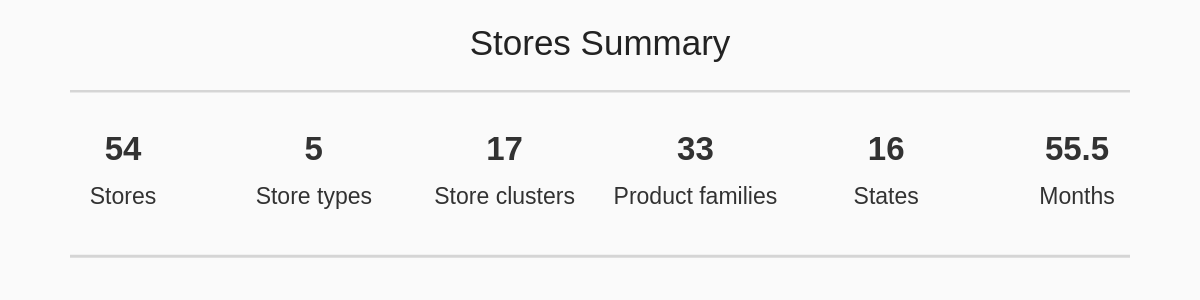
\includegraphics[width=0.9\textwidth]{plots/data_description/stores_summary.png}
  \caption[Summary of the training dataset]{\textbf{Summary of the training dataset}. The cluster information denotes similarity between stores.}
  \label{fig:store_summary}
\end{figure}

\section[Data exploration and data cleaning]{Data exploration and data cleaning}
\label{sec:eda}

Performing an exploratory data analysis (eda) of the sales from the training dataset, we can observe that grocery I, beverages, and produce are the top 3 most consumed products (see \autoref{fig:eda}) . Additionally, store type A, and cluster 5 are the most frequent among their classification.

\begin{figure}[!htb]
  \centering
  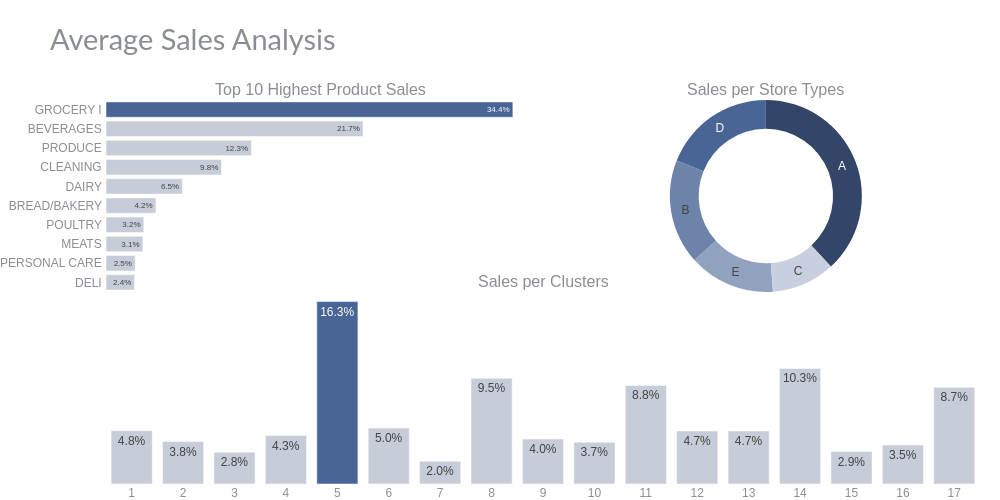
\includegraphics[width=0.9\textwidth]{plots/eda/sale_analysis.png}
  \caption[EDA of sales]{\textbf{EDA of sales}. The plot describes the sales by product, store type, and per cluster (left, right, and below, respectively). Darker blue represents higher sales. }
  \label{fig:eda}
\end{figure}

\subsection[Stationarity and seasonality analyses]{Stationarity and seasonality analyses}
\label{sec:st_s_analysis}

The sales represented by \autoref{fig:target} shows low-peaks at the end of each year, which is explained because the stores are closed at new years. Moreover, we can observe a pattern at each year, with increased sales at the end of the year which overlaps with the Christmas eves, suggesting a seasonal pattern. These patterns are highlighted after smoothing the sales data  with a 7 days moving average (the continuous red lines from the \autoref{fig:target}).

\begin{figure}[!htb]
  \centering
  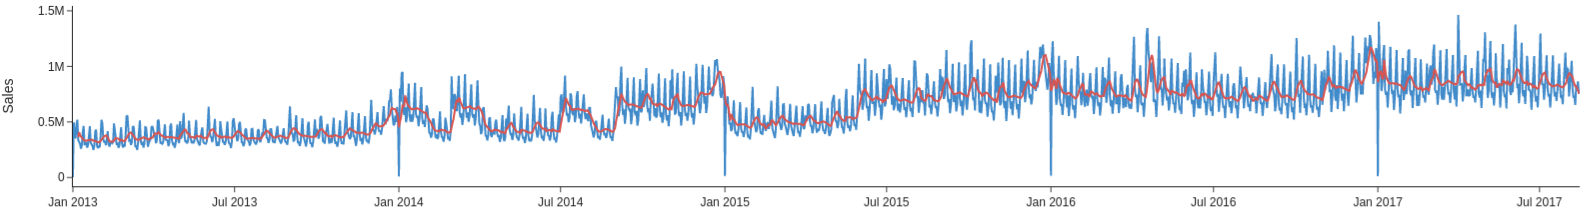
\includegraphics[width=0.9\textwidth]{plots/eda/target-time-series-plot-DF-testProc.png}
  \caption[Target time series data]{\textbf{Target time series data}. The y-axis represents the training sales from 2013-01-01 to 2017-08-15, and the x-axis shows the time in days (1,087 days). The sales were aggregated by all stores and products (see \autoref{fig:store_summary}). The raw data, and smoothed data (7 days moving average) are denoted by the continuous blue, and red lines, respectively.}
  \label{fig:target}
\end{figure}

The stationary and seasonality are key components to select the adequate machine learning model (such as ARIMA, SARIMA, etc.) to generate reliable forecasting. A stationary time series is defined, if their statistical properties such as mean, and variance are all constant, and independent of time. In consequence, we implemented a \textit{Dickey-Fuller test} to assess stationarity. We obtained a \textit{p-value} of 0.09, using a significance level of 0.05, we can reject the null hypothesis (the series is stationary) concluding that our series is non-stationarity. Obtaining valuable information about which models are more suitable.

\begin{figure}[!htb]
  \centering
  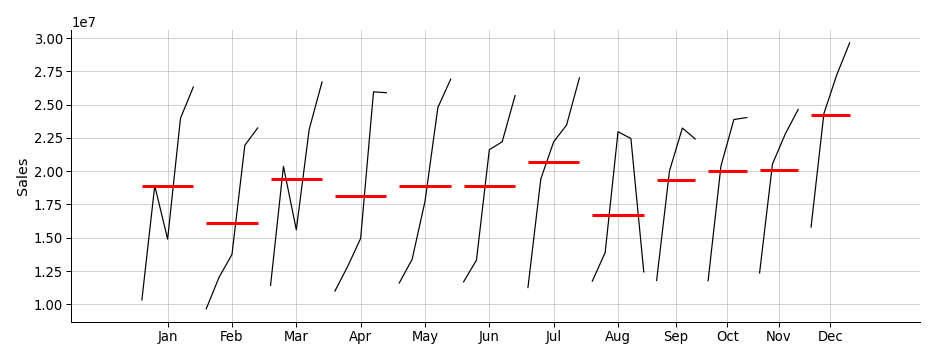
\includegraphics[width=0.9\textwidth]{plots/eda/seasonal_analysis.png}
  \caption[Analysis of seasonality]{\textbf{Analysis of seasonality}. The y-axis represents the sales aggregated by month, x-axis shows the analyzed months (from January to December), the horizontal red lines denote the sales average by month (55.5 months).}
  \label{fig:target}
\end{figure}




\subsection[Time series Decomposition]{Time series Decomposition}
\label{sec:decomposition}


